\subsection{Architecture}\label{sub:architecture}
ECDAR consists of four major systems as seen in \autoref{fig:ECDAR-architecture}.
There are the two engines, Reveaal and j-Ecdar, as well as the ECDAR GUI, and a test framework as seen in \autoref{fig:ECDAR-architecture}. 
The GUI and the engines communicate through Protocol Buffers (Protobuf) and gRPC (\textbf{G}oogle \textbf{R}emote \textbf{P}rocedure \textbf{C}all) as indicated by the arrows.
\begin{figure}[H]
    \centering
    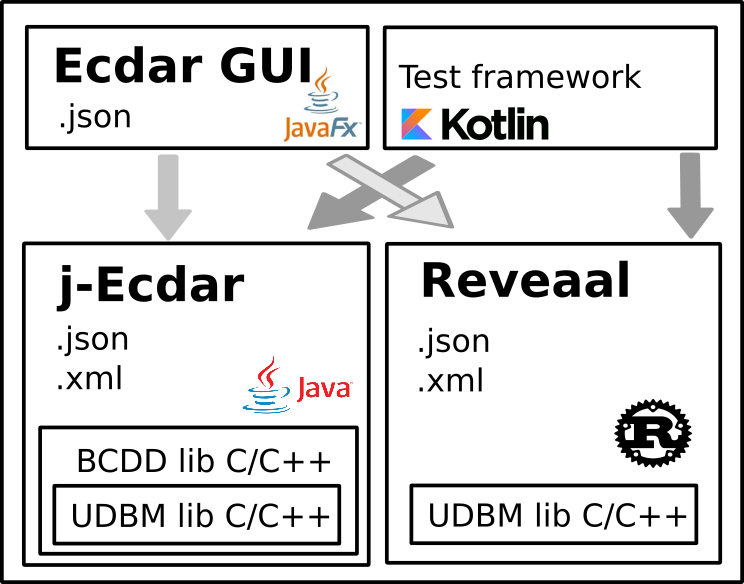
\includegraphics[width=0.75\textwidth]{common/figures/ArchOverview.png}
    \caption{The architecture of ECDAR visualized \cite{ECDARNET}.}
    \label{fig:ECDAR-architecture}
\end{figure}
% Figure old, get new

The graphical user interface (\textbf{GUI}) is written in JavaFX \cite{ECDARNET}  which is a graphics and media library for Java. 
The interface provides the tools which enables the user to model their real time systems. The GUI sends queries to the engines through gRPC using Protobuf. 
%This is illustrated by the arrows going from the Ecdar GUI component to the j-Ecdar and Reveaal components, as seen in \autoref{fig:ECDAR-architecture}. 
The gRPC and Protobuf frameworks have the advantage of being cross platform and work across languages \cite{gRPC}\cite{google_protocol_nodate}, simplifying the integration process and making it easy to use.

ECDAR runs on two verification engines: j-Ecdar and Reveaal. 
The purpose of having two different engines is to make the whole platform more reliable. 
With two engines their results can be compared which will help ensure correctness in both engines.
The j-Ecdar component is an engine written in Java.
The main priorities for this engine are readability and correctness, and, as stated on ECDAR's homepage: "no effort is put into optimizing the code for speed" \cite{ECDARNET}.
In contrast to this, the Reveaal engine is intended to be fast and parallelizable. 
Recently, the libraries which the engine uses have been rewritten in Rust from C/C++, with the intention of implementing multithreading. 

ECDAR makes use of a testing framework written in Kotlin. 
The testing framework uses a collection of test cases to test both of the engines. 
The testing framework is vital to perform conformance testing between j-Ecdar and Reveaal as well as automated performance testing and hand-designed test cases. 